\documentclass[8pt,a4paper]{article}
\usepackage[utf8]{inputenc}
\usepackage{graphicx}
\graphicspath{ {./images/} }

\usepackage{color}   
\usepackage{hyperref}
\usepackage{listings}
\usepackage[utf8]{inputenc}
\usepackage{amsmath}
\usepackage{amsfonts}
\usepackage{amsthm}
\usepackage{german}

\usepackage[onehalfspacing]{setspace}


\let\stdsection\section
\setlength{\parindent}{0in} 


% Useful packages
\usepackage{amsmath}
\usepackage{graphicx}
\usepackage[colorlinks=true, allcolors=blue]{hyperref}
\title{Neuronale Netze in der Bildverarbeitung Versuch-1}
\author{Julian Schmidt, Vincenz Forkel}

\begin{document}
\maketitle
\newpage
\tableofcontents
\newpage
\section{Einführung}
Ziel des ersten Versuchs des Praktikums Neuronale Netze in der Bildverarbeitung im Wintersemester 2021/22 ist es Grundlagen des Aufbaus und der Arbeit mit Neuronalen Netzen kennen zu lernen.\\
Konkret wird hier der MNIST-Datensatz verwendet, für den ein Neuronales Netz darauf trainiert werden soll Ziffern zwischen 0 und 9 zu klassifizieren.\\

Der MNIST (Modified National Institute of Standards and Technology database) ist eine öffentlich verfügbare Datenbank von handgeschriebenen Ziffern.\\
Wobei jede Ziffer als 28 × 28 Pixel großes Graustufen-Bild gespeichert ist.\\

Verwendet wird hierfür die Skript Sprache Matlab.\\

alle Skripte und Lösungen befinden sich in diesem Github Repository:\\
https://github.com/JulianSchmidt96/MessTechnikPraktikumNN/
\newpage
\section{Netzwerk Architektur}\label{architektur}
Um die Architektur des Netzwerkes zu erstellen wurde die Matlab-Toolbox für Neuronale Netze verwendet.

\lstinputlisting{layers.m}
\\
Wie hier zu sehen ist besteht das Netz aus zwei 'fully connected layer', einem 'relu layer', einem 'softmax layer' und einem 'classification layer'.
\\
\\

\begin{center}
    

    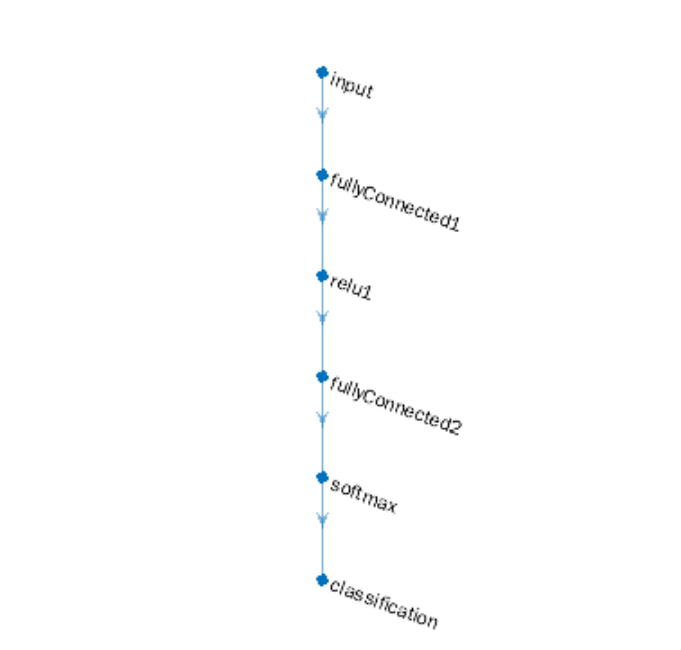
\includegraphics[scale = 0.4]{model.png}
    \caption{Netz Architektur}
\end{center}


\section{Aufgaben}
\subsection{Aufgabe 1}
\subsubsection{Aufgabenstellung}
\\
1. Nutzen Sie die gegebene Matlab-Vorlage und laden Sie Bilder und Labels aus dem MNIST-Datensatz. Teilen Sie die Daten in Trainings- und
Validationsdaten auf.
\\
\subsubsection{Lösung}
\\
Die Daten werden aus der Neuronale Netze Toolbox Bibliothek geladen.\\
aus 1000 geladenen Daten werden 750 für Trainings-Daten und 250 für Validierungs-Daten verwendet

\\

\lstinputlisting{dataset.m}

\\

\subsection{Aufgabe2}
\\
\subsubsection{Aufgabenstellung}
\\
Erstellen Sie ein neuronales Netz zur Bildklassifizierung. Dieses sollte zum Beispiel aus einem Image input layer, einem Fully connected
layer, einem ReLU layer, einem weiteren Fully connected layer, einem Softmax layer und einem Classification layer (nur bei Verwendung der Funktion trainNetwork) bestehen. Achten Sie darauf, dass
das Softmax-Layer einen Vektor mit einer Länge entsprechend der zu
erkennenden Klassen benötigt, um die Klassifizierung zu ermöglichen.
Benutzen Sie den Befehl analyzeNetwork, um ihre Struktur auf Fehler
zu prüfen. Legen Sie dann die Hyperparameter für das Training fest.
\\
\subsubsection{Lösung}
\\
Prinzipiell geh es hier bei um die Netzwerkarchitektur, welche bereits in Abschnitt 2 erläutert.

\\
\subsection{Aufgabe 3}
\\
\subsubsection{Aufgabenstellung}
Trainieren Sie das neuronale Netz mit der Funktion trainNetwork oder
mit einer eigenen Trainingsschleife. Es ist wünschenswert, wenn Sie
beide Varianten ausprobieren. Bei korrekter Implementierung werden
beide Wege funktionieren und zu vergleichbaren Ergebnissen führen.
Jedoch können Sie bei der erfolgreichen Implementierung einer benutzerdefinierten Trainingsschleife ein umfangreiches Verständnis zum
Training Neuronaler Netze gewinnen. Nutzen Sie zunächst für beide
Optionen den Solver Adam und evaluieren Sie das Ergebnis, indem Sie
das Netz anhand der Validierungsdaten testen. Mit geeigneten Parametern sollte es möglich sein, eine Genauigkeit von mindestens 95 %
zu erreichen.\\
\subsubsection{Lösung}
\\
Hierfür werden relevante Trainingsoptionen in der Variable 'modelOptions zwischengespeichert.
\\
\lstinputlisting{options.m}
\\
Mit dem Optimizer Adam lies sich bei einer Trainingsdauer von 30 Epochen eine finale Validierungsgenauigkeit von ca. 98 Prozent erreichen.
\\
\subsection{Aufgabe 4}
\\
\subsubsection{Aufgabenstellung}
\\Ermitteln Sie die mittlere Klassifizierungsgenauigkeit des NN in Ab-
hängigkeit der eingelesenen Ziffern.

Stellen Sie das Ergebnis in einem geeigneten Diagramm (µ = f (Ziffer))
dar
\subsubsection{Lösung}
\subsection{Aufgabe 5}
\\
\subsubsection{Aufgabenstellung}
\\
Vergleichen Sie nun die beiden Solver Adam und Sgdm mit mindestens 6
verschiedenen Lernraten zwischen 10−6 und 10−1 . Stellen Sie die er-
reichte mittlere Klassifizierungsgenauigkeit in Abhängigkeit von der
Lernrate dar und verwenden Sie für die Lernrate eine logarithmische
Achse.
\\
\subsubsection{Lösung}
in zwei for-schleifen werden beide optimizier mit den verschiedenen Lernraten und sonst gleichen parametern getestet und es werden Lernrate+Optimizer mit der höchsten finalen Genauigkeit übernommen.
\lstinputlisting{findlr.m}


\subAufgabe{6}
\subsection{Aufgabenstellung}
Testen Sie außerdem mindestens 5 verschiedene Größen des Mini-Batch
zwischen 16 und 256. Wählen Sie aus der vorherigen Aufgabe eine Lern-
rate aus, bei der der Trainingsprozess zu einer hohen Klassifizierungs-
genauigkeit konvergiert. Stellen Sie die mittlere Klassifizierungsgenau-
igkeit und die benötigte Trainingszeit in Abhängigkeit von der Größe
des Mini-Batches dar.
\\

\subsection{Lösung}
Es wird ein Array aus 5 verschiedenen Minibatchgrößen erstllt und dann wird das Netz in einer for-schlefe mit jeder Minibatch-Größe erneut trainiert, hierbei wird verglichen welche Minibatch-Größe die geringste Trainingszeit besitzt.

\lstinputlisting{findmbatch.m}

\subsection{Aufgabe 7}
\subsubsection{Aufgabenstellung}
Leiten Sie aus den Trainingsergebnissen Zusammenhänge zwischen den
untersuchten Hyperparametern und der Trainingszeit sowie der erreichten Genauigkeit bei der Klassifizierung ab. Formulieren Sie hierfür eine
kurze Diskussion.
\subsubsection{Lösung}
Es hat sich eindeutig gezeigt, dass Adam ein genauerer Optimizer als SGDM ist.

Die Lernrate scheint ebenfalls einen großen Einfluss auf die Genauigkeit des Netzes zu haben.
Auch wenn sich die Genauigkeit beinahe durchgehend in einem Bereich größer 90 Prozent befindet lässt sich die Genauigkeit immernoch etwas verbessern durch das durchprobieren verschiedener Lernraten.
Hierbei wurden die Lernraten jeweils um den Faktor 10 verändert.\\

Testweise haben wir in einem großem Durchlauf einmal den Lernratenarray so angepasst das wir ca 50 verschiedene Lernraten getestet haben.\\
Hierfür muss lediglich der lernratenarray angepaßt werden, das Skript findet selbstständig die ideale Lernrate.
Zu Beachten ist allerdings, dass hier für eine sehr lange Laufzeit eingeplant werden muss.\\

Wir haben hierfür einmal das Skript über ein Wochenende laufen lassen.

Eine geschickte Anpassung der Minibatch-Größen würde die Trainings-Dauer und somit Gesamtlaufzeit verringern.

Die Ergebnisse haben gezeigt, dass Änderungen der Minibatch-Größe einen direkten Einfluss auf die Laufzeit hat.\\
Beim Testen hat sich gezeigt, dass für verschiedene Minibatch-Größe unterschiedliche Genauigkeiten erreicht wurden.\\
Das liegt allerdings mit hoher Wahrscheinlichkeit da dran, dass jede Prädiktion auf statistischen Größen basiert.\\
Wenn ein Neuronales Netz mehrfach mit exakt gleichen Parametern trainiert wird, ist es  unmöglich immer zu 100 Prozent das gleiche Ergebnis zu erhalten.
\end{document}
